% $Header: /home/vedranm/bitbucket/beamer/solutions/generic-talks/generic-ornate-15min-45min.de.tex,v 90e850259b8b 2007/01/28 20:48:30 tantau $

\documentclass{beamer}

% Diese Datei enth�lt eine L�sungsvorlage f�r:


% - Vortr�ge �ber ein beliebiges Thema.
% - Vortragsl�nge zwischen 15 und 45 Minuten. 
% - Aussehen des Vortrags ist verschn�rkelt/dekorativ.



% Copyright 2004 by Till Tantau .
%
% In principle, this file can be redistributed and/or modified under
% the terms of the GNU Public License, version 2.
%
% However, this file is supposed to be a template to be modified
% for your own needs. For this reason, if you use this file as a
% template and not specifically distribute it as part of a another
% package/program, I grant the extra permission to freely copy and
% modify this file as you see fit and even to delete this copyright
% notice. 



\mode<presentation>
{
  \usetheme{Frankfurt}
  \setbeamertemplate{footline}[page number]
%   \usetheme{Rochester}
  % oder ...
  %\usecolortheme{crane}
  
  \setbeamercovered{transparent}
  % oder auch nicht
}
\setbeamercolor{alerted text}{fg=green!40!black}

\usepackage[english]{babel}
% oder was auch immer

\usepackage[latin1]{inputenc}
% oder was auch immer
\usepackage{amsmath}
\usepackage{times}
\usepackage[T1]{fontenc}
% Oder was auch immer. Zu beachten ist, das Font und Encoding passen
% m�ssen. Falls T1 nicht funktioniert, kann man versuchen, die Zeile
% mit fontenc zu l�schen.
\usepackage{booktabs}
\usepackage{multirow}
\newcommand{\T}{\ensuremath{^\mathsf{T}}}

\title % (optional, nur bei langen Titeln n�tig)
{Ultrakurze Laserpulse:}

\subtitle
{wie sie helfen die Geheimnisse heterogener Katalyse zu entschl�sseln} % (optional)

\author[] % (optional, nur bei vielen Autoren)
{Robert Scholz}
% - Der \inst{?} Befehl sollte nur verwendet werden, wenn die Autoren
%   unterschiedlichen Instituten angeh�ren.

\institute % (optional, aber oft n�tig)
{AG Saalfrank \\ Institut f�r Chemie \\ Universit�t Potsdam}

%   \inst{1}%
%   Institut f�r Informatik\\
%   Universit�t Hier
%   \and
%   \inst{2}%
%   Institut f�r theoretische Philosophie\\
%   Universit�t Dort}
% - Der \inst{?} Befehl sollte nur verwendet werden, wenn die Autoren
%   unterschiedlichen Instituten angeh�ren.
% - Keep it simple, niemand interessiert sich f�r die genau Adresse.

\date[] % (optional)
{19. April 2017}


%\subject{Informatik}
% Dies wird lediglich in den PDF Informationskatalog einf�gt. Kann gut
% weggelassen werden.


% Falls eine Logodatei namens "university-logo-filename.xxx" vorhanden
% ist, wobei xxx ein von latex bzw. pdflatex lesbares Graphikformat
% ist, so kann man wie folgt ein Logo einf�gen:





% Folgendes sollte gel�scht werden, wenn man nicht am Anfang jedes
% Unterabschnitts die Gliederung nochmal sehen m�chte.
% \AtBeginSubsection[]
% {
%   \begin{frame}[plain]{Outline}
%     \tableofcontents[currentsection,currentsubsection]
%   \end{frame}
% }


% Falls Aufz�hlungen immer schrittweise gezeigt werden sollen, kann
% folgendes Kommando benutzt werden:

%\beamerdefaultoverlayspecification{<+->}



\begin{document}



\begin{frame}[plain]
  \titlepage

\end{frame}

\begin{frame}{Motivation}
 \begin{block}{Heterogene Katalyse}
  
 \end{block}

\end{frame}

\begin{frame}[plain]{Outline}
  \tableofcontents
  % Die Option [pausesections] k�nnte n�tzlich sein.
\end{frame}



% Da dies ein Vorlage f�r beliebige Vortr�ge ist, lassen sich kaum
% allgemeine Regeln zur Strukturierung angeben. Da die Vorlage f�r
% einen Vortrag zwischen 15 und 45 Minuten gedacht ist, f�hrt man aber
% mit folgenden Regeln oft gut.  

% - Es sollte genau zwei oder drei Abschnitte geben (neben der
%   Zusammenfassung). 
% - *H�chstens* drei Unterabschnitte pro Abschnitt.
% - Pro Rahmen sollte man zwischen 30s und 2min reden. Es sollte also
%   15 bis 30 Rahmen geben.

\section{Introduction}
  \subsection[Motivation]{Motivation - in general and system specific}
  
\begin{frame}{General motivation}
%   \begin{columns}[t]
%   \column{.7\textwidth}
    \begin{block}{Why investigate fs-laser-driven surface dynamics?}
      \begin{itemize}
      \item gain fundamental understanding of adsorbate bonding \newline $\Rightarrow$ additional tool besides scattering experiments and STM
      \item possible direct application in catalysis: ``femtochemistry'' \newline $\Rightarrow$ new reaction pathways opened up by fs-lasers  
      \end{itemize}
    \end{block}
%   \column{.3\textwidth}
%     \begin{block}{}  

      \begin{figure}
	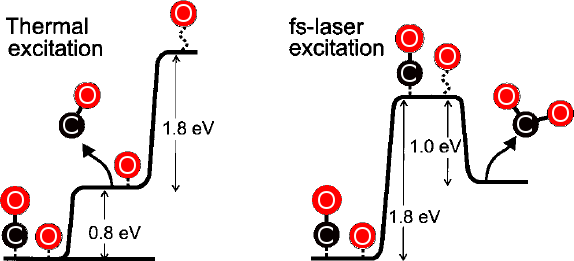
\includegraphics[width=.65\textwidth]{figures/CO_CO2.png}
      \end{figure}\vspace{-.5cm}                  
    \begin{center}  		
	\begin{footnotesize}CO/O-coadsorbate @ Ru(0001)\end{footnotesize} \\ \begin{scriptsize}M. Bonn \textit{et al.}, \textit{Science} 1999 \end{scriptsize}
    \end{center}
      
%     \end{block}
%   \end{columns}  
\end{frame}

% \begin{frame}{CO/Ru-System}


\begin{frame}{Specific motivation for investigating CO/Ru(0001)}
  \begin{block}{CO/Ru(0001) system important for catalysis, e.g.:}
	\begin{itemize}
	  \item Fischer-Tropsch synthesis {($n\,$CO + 2$n\,$H$_2 \rightarrow$ Alkane/Alkene/Alkohole + H$_2$O)} 
	  \item exhaust gas converters \begin{footnotesize} (cars, power plants, etc.)	                                               \end{footnotesize}
	\end{itemize}

  \end{block}
 
  \begin{block}{Experimentally well studied system}
    \begin{itemize}
	  \item especially regarding fs-laser irradiation:\begin{itemize}\item \begin{scriptsize}e.g. Bonn \textit{et al.}, \textit{Science} 1999; Funk \textit{et al.}, \textit{JChemPhys} 2000\end{scriptsize}	                                                                                                                                                      \item\begin{footnotesize}(both Ertl group $\Rightarrow$ chemistry Nobel prize 2007).	                                                                                                                                                                                                                                                                                                                                        \end{footnotesize}\end{itemize}
	  \item desorption kinetics: large prefactors $\Rightarrow$ still not understood 
	  \item recently, time resolved x-ray spectra (XAS and XES)
	  \newline $\Rightarrow$ ``movie'' of changes in orbital density of states
	  \begin{itemize}
	    \item {\scriptsize Dell'Angela \textit{et al.}, \textit{Science} 2013}
	  \end{itemize}

	  
%      \item Ultrafast time-resolved X-Ray-spectroscopy hints to physisorbed precursor state
%      \item Recent full 6D PES does not feature physisorption well
    \end{itemize}
  \end{block}
  
%   \begin{block}{Open questions for theory}
%     \begin{itemize}
%      \item Do dynamics reproduce other observables correctly? (e. g. desorption yield) 
%      \item Can the X-Ray-spectra also be explained without physisorption?
%     \end{itemize}
%   \end{block}
\end{frame}

\begin{frame}{Further specific motivation for investigating CO/Ru}{F\"uchsel \textit{et al.}, \textit{JChemPhys} 2014} 
  \vspace*{-.4cm}
  \begin{columns}
	\column{.5\textwidth}
	  \begin{figure}
		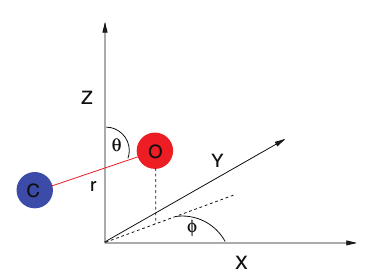
\includegraphics[width=.8\textwidth]{figures/6dimScheme.png}
	  \end{figure}
	\column{.5\textwidth}
	  \begin{figure}
		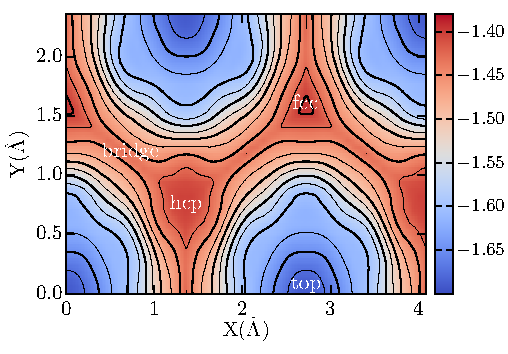
\includegraphics[width=.8\textwidth]{figures/PES_XYview.pdf}
	  \end{figure}
	
  \end{columns}
  \begin{block}{Important prior theory work was done at our group \newline{\scriptsize F\"uchsel \textit{et al.}, \textit{JChemPhys} 2014}}
  \begin{itemize} 
    \item Development of a potential energy surface (PES)
	  \begin{itemize}
	    \item \footnotesize from over 90$\,$000 DFT points!
	        \item all 6 dimensions of the adsorbate
    \item very fast because preconstucted\\~
    \item[\LARGE$\Rightarrow$] {\large\textbf{enables large-scale dynamics!}}
    	  \end{itemize}
  \end{itemize}
  \end{block}
\end{frame}


\subsection[101 of fs-lasers]{First impressions of fs-laser-driven dynamics}



\begin{frame}{What happens after fs-laser excitation of the metal?}
%   \begin{figure}
	\hspace*{-.5cm}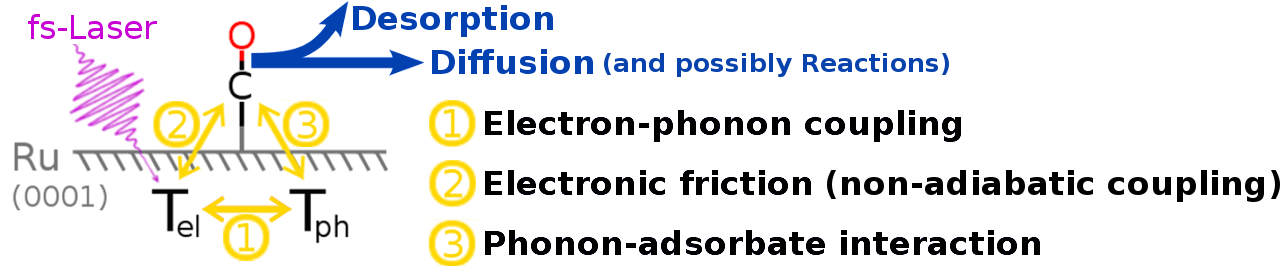
\includegraphics[width=1.1\textwidth]{figures/modifiedSurfScheme.png} 
%   \end{figure}

  \begin{columns}
  \column{0.8\textwidth}
  \begin{block}{Coupling between 3 kinds of degrees of freedom:} 
    \begin{itemize}                                                                   
      \item electron gas ($T_\mathrm{el}$) 
	\begin{itemize}
	  \footnotesize
	 \item initially absorbs laser energy
	 \item low heat capacity $\Rightarrow$ high $T_\mathrm{el}$ ($\approx$5-10$\,$kK)
	\end{itemize}
      \item lattice vibrations ($T_\mathrm{ph}$)
			\begin{itemize}
	  \footnotesize
	 \item thermalization with electrons: ps time scale
	 \newline $\Rightarrow$ fs-laser causes two distinct temperatures!
	\end{itemize}
      \item adsorbate movement ($T_\mathrm{ads}$)
    \end{itemize}

  \end{block}
  \column{0.2\textwidth}
  \begin{figure}
    \hspace*{-.2cm}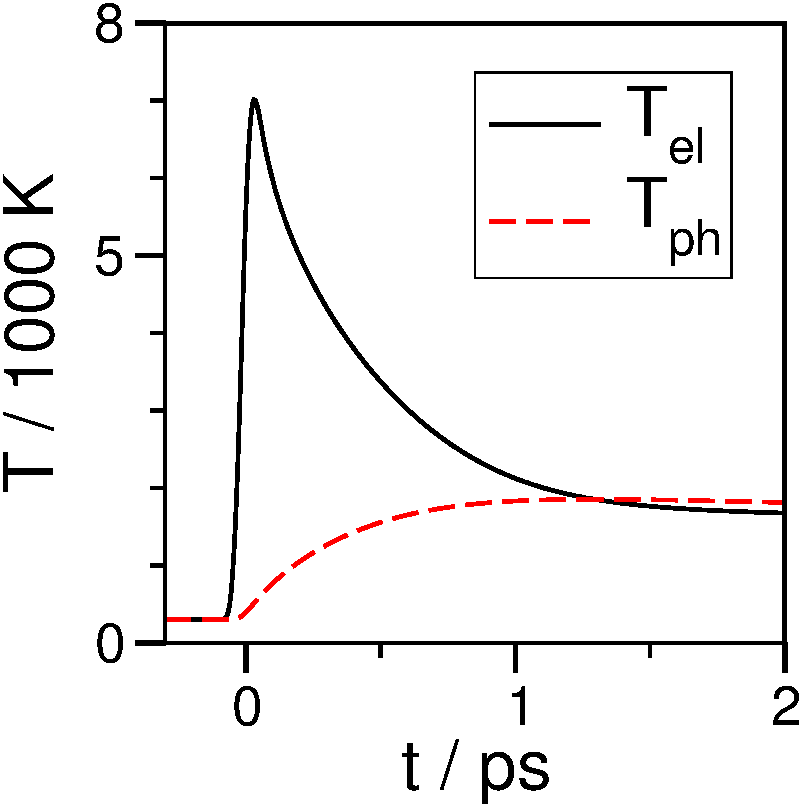
\includegraphics[width=1.3\textwidth]{figures/TTM_1pulse-eps-converted-to.pdf}
  \end{figure}
  \end{columns}
\end{frame}

\begin{frame}{Details of the time-resolved x-ray experiment}{Dell'Angela \textit{et al.}, \textit{Science} 2013 {\scriptsize (experimental part by Nilsson group, SLAC/LCLS, Stanford)}}
  \vspace*{-.7cm}
  \begin{columns}[t]
    \column{0.51\textwidth}
      \begin{block}{What was done?}
        \begin{itemize}
         \item pump: \textit{vis}-fs-laser 
         \item probe: x-ray free $e^{-}$ laser
		  \begin{itemize}\footnotesize
		    \item K-edge of O-atom
		  \end{itemize} 
        \end{itemize}

      \end{block}
%       \begin{block}{How does it work?}
%        
%       \end{block}	  
      \begin{block}{What is observed?}
        \begin{itemize}
	  \item orbital density of states at O 
	  \item energies shift towards gas-phase values of CO
	  \item intensities change 
	  \begin{itemize}
		\footnotesize
	   \item 2$\tilde{\pi}^*$ $\Rightarrow$ increase by $\sim30$\% 
	   \item \~{d}$_\pi$ $\,\Rightarrow$ decrease by $\sim30$\%
	   \item participator peak appears
	  \end{itemize}
	  \large \item[\LARGE$\Rightarrow$] physisorbed precursor(?)
	\end{itemize}	  
      \end{block}      
    \column{0.50\textwidth}
     \vspace*{-.8cm}
  \begin{figure}
    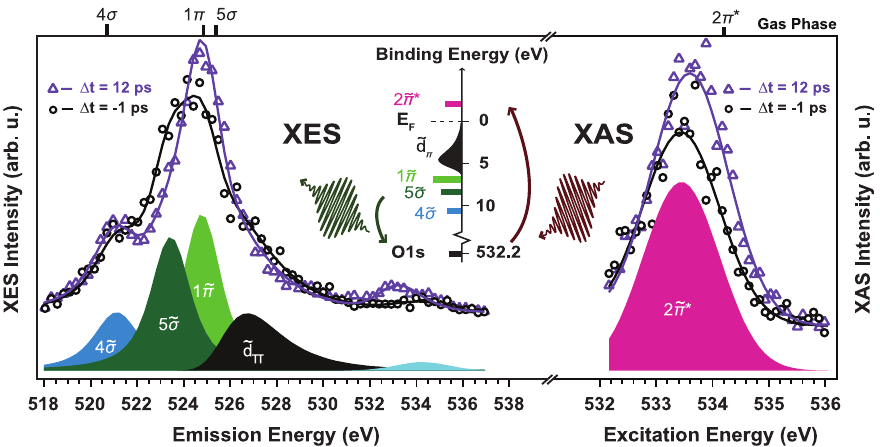
\includegraphics[width=1.1\textwidth]{figures/scienceXray.png}
  \end{figure}
         \vspace*{-.15cm}
%   \begin{figure}
    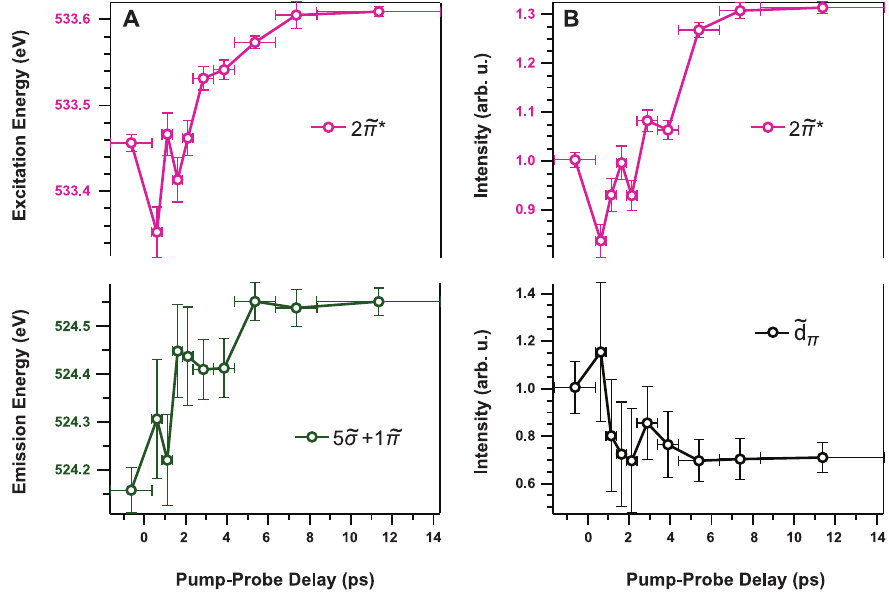
\includegraphics[width=1.1\textwidth]{figures/XrayIntOverTime.png}
%   \end{6figure}
  \end{columns}
\end{frame}

\begin{frame}{Details of the accompanying theory}{still Dell'Angela \textit{et al.}, \textit{Science} 2013 {\scriptsize (theory part by N\o{}rskov group, SUNCAT, Stanford)}}
  	\vspace{-1cm}
  \begin{columns}[t]
  \column{0.55\textwidth}
	\vspace{-.53cm}
	\begin{figure}
	  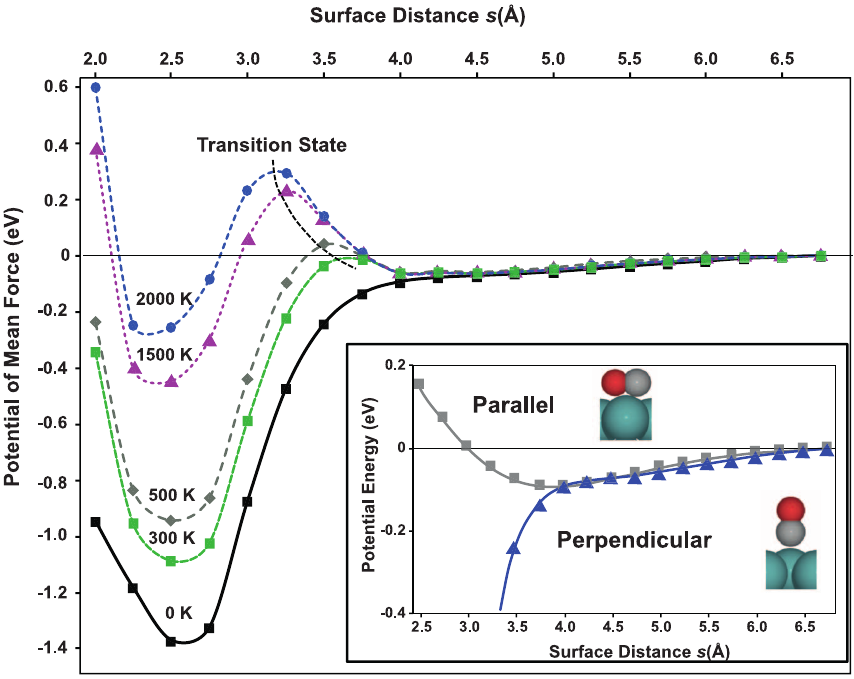
\includegraphics[width=1.06\textwidth]{figures/sciencePMF.png}
	\end{figure}
	\vspace{.21cm}
	{\scriptsize \begin{center}
Dell'Angela \textit{et al.}, \textit{Science} 2013	                                                               \end{center}}
  \column{0.45\textwidth}
	\begin{figure}
	  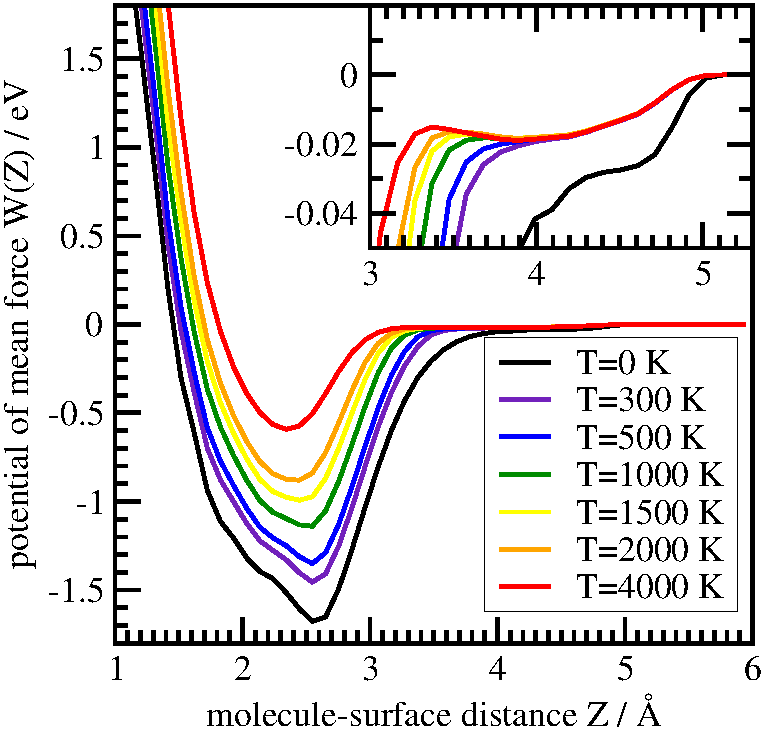
\includegraphics[width=1.1\textwidth]{figures/GernotPMF.pdf}
	\end{figure}
	{\scriptsize \begin{center}
Scholz \textit{et al.}, \textit{PhysRevB} 2016	                                                           \end{center}}
  \end{columns}


\end{frame}



\section{Models and methods}

% \subsection{The foundation: our 6D potential energy surface (PES)}
\subsection[6D PES and TTM]{Foundations: 6D potential and two-temperature model}
\begin{frame}{More facts about the potential energy surface (PES)}
  \begin{columns}
   \column{0.9\textwidth}
     
  \begin{block}{How was it constructed?}
    \begin{itemize}
      \item GGA-level (RPBE) with VdW-correction (D2)

      \item (2x2) cell with 1 CO $\Rightarrow$ 14 atoms, 0.25 ML coverage
      \begin{itemize}
	\item \footnotesize all 6 dimensions of adsorbate $\Rightarrow$ surface atoms frozen
      \end{itemize} 
      \item interpolation with cubic splines and\newline corrugation reducing procedure (CRP)
      \begin{itemize}
	\item \footnotesize atomic potentials temporarily substracted \newline $\Rightarrow$ smoother intermittent potential, interpolates better
      \end{itemize}
      \item slightly newer PES: C$_{3v}$- instead of C$_{6v}$-symmetry	
      \begin{itemize}
	\item \footnotesize differences between hcp and fcc sites not neglected
      \end{itemize}
     \end{itemize}

  \end{block}

   \column{0.15\textwidth}
       \begin{figure}
	\hspace*{-.2cm}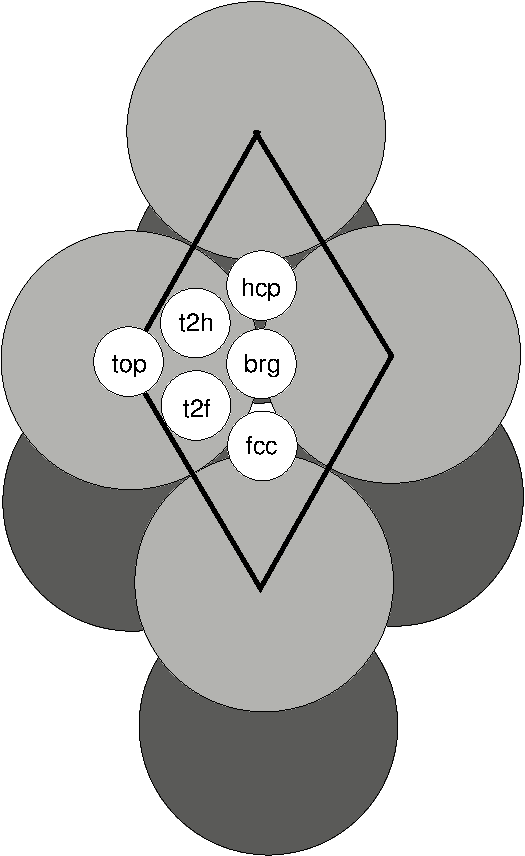
\includegraphics[width=1.3\textwidth]{figures/PES_samplepoints.pdf}
      \end{figure}
      
%       \begin{figure}
% 	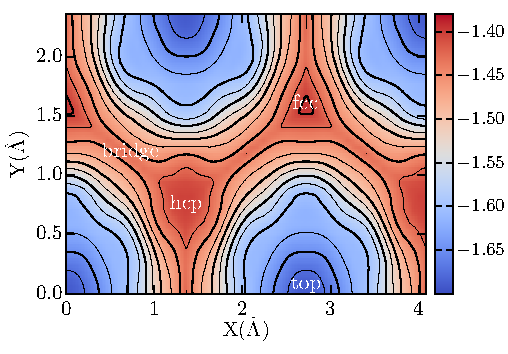
\includegraphics[width=1.2\textwidth]{figures/PES_XYview.pdf}
%       \end{figure}

  \end{columns}
        \begin{figure}
	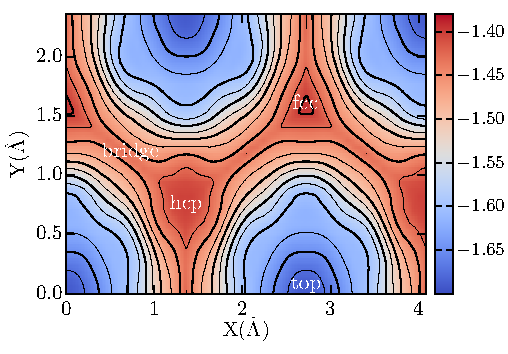
\includegraphics[width=0.33\textwidth]{figures/PES_XYview.pdf}
      \end{figure}
\end{frame}

% \subsection{The two-temperature model (TTM)}
\begin{frame}{Two-temperature model (TTM)}{Two coupled heat diffusion equations}
  
  \begin{columns}
   \column{0.3\textwidth}
    \begin{figure}
	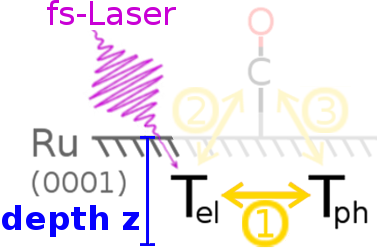
\includegraphics[width=1\textwidth]{figures/Part1SurfScheme.png}
  \end{figure}
         \begin{figure}
    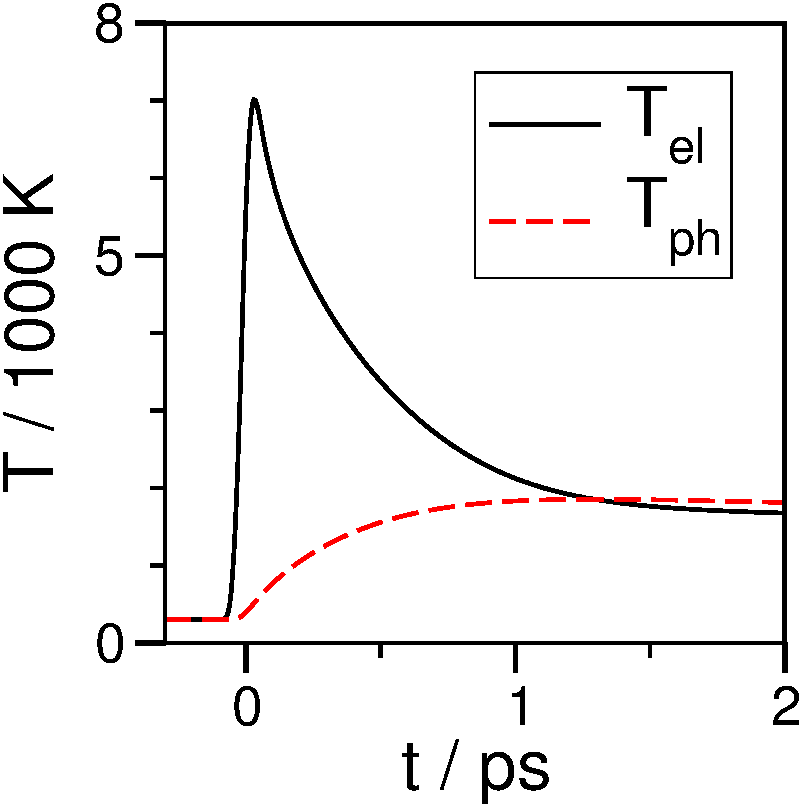
\includegraphics[width=1\textwidth]{figures/TTM_1pulse-eps-converted-to.pdf}
  \end{figure} 
  \column{0.8\textwidth}
  \vspace*{-1cm}
  \begin{figure}
	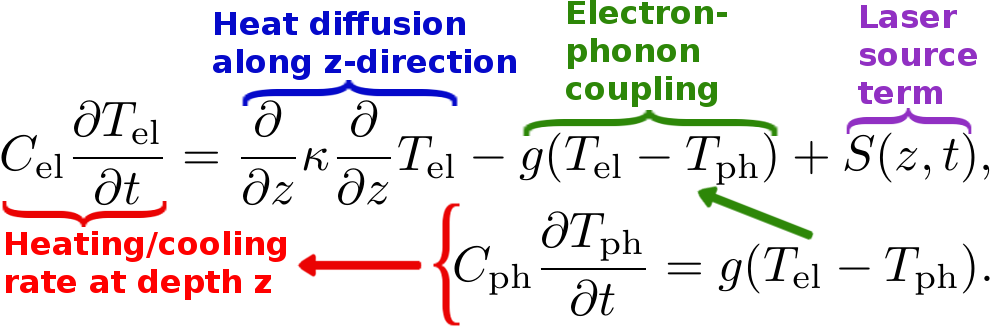
\includegraphics[width=\textwidth]{figures/2TM_equs.png}
  \end{figure}  
   \begin{block}{Original TTM {(\scriptsize Anisimov \textit{et al.}, \textit{SovPhys-JETP} 1974)} }
    \begin{itemize}
     \item $T_\mathrm{el}$ and $T_\mathrm{ph}$ as $f(z,t)$ {\footnotesize from laser/material properties}
     \begin{itemize}
     \footnotesize
     \item $C_\mathrm{el}$ and $C_\mathrm{ph}$ $\Rightarrow$ heat capacities
     \item $\kappa = \kappa_0 \frac{T_\mathrm{el}}{T_\mathrm{ph}}$ $\Rightarrow$ electron heat conductivity
     \item $g$ $\Rightarrow$ electron-phonon coupling constant
     \item $S(z,t)$ $\Rightarrow$ depends on pulse shape, $\lambda$, fluence $F$ 
          \end{itemize}
    \end{itemize}

   \end{block}
  \end{columns}




\end{frame}


\subsection[MDEF]{Electronic friction: non-adiabatic coupling approximated}
\begin{frame}{Different approaches to non-adiabatic coupling}
  \begin{figure}
	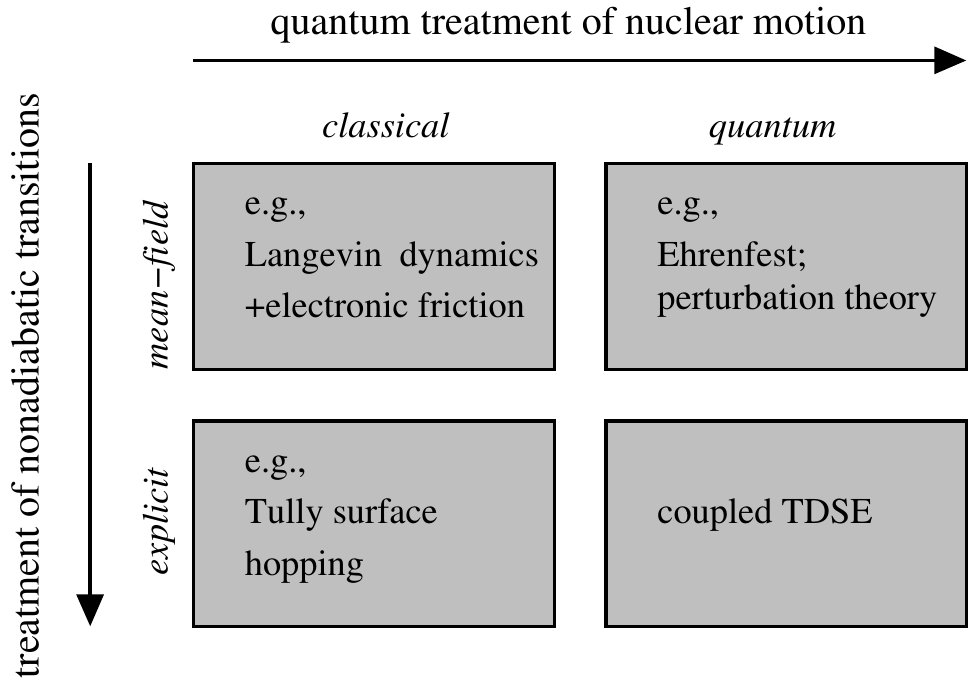
\includegraphics[width=.6\textwidth]{figures/scheme_nonadiab.png}
  \end{figure}
  \begin{block}{Langevin dynamics + electronic friction}
   \begin{itemize}
    \item fastest method $\Rightarrow$ suited for multi-dimensional dynamics
    \item good approximation for weak non-adiabatic coupling
   \end{itemize}

  \end{block}

\end{frame}

\begin{frame}{The Langevin equation}{A stochastic differential equation}
  \begin{columns}
  \column{0.3\textwidth}
   \begin{figure}
	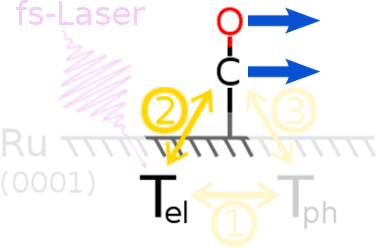
\includegraphics[width=\textwidth]{figures/Part2SurfScheme.png}
  \end{figure}
  \column{0.8\textwidth}
\begin{figure}
	
\includegraphics[width=\textwidth]{figures/Langevin_eq.png}
  \end{figure}
    \end{columns}
  \begin{block}{Langevin equation within IAA {\small(independent atom approx.)}}
  \begin{itemize}
   \item friction coefficient of Atom k: $\eta_{\mathrm{el},k}(\underline{r}_k)$ $\Rightarrow$ dissipation
  
      \begin{itemize}
      \footnotesize
      \item derived from local density friction approximation (LDFA)
      \newline $\Rightarrow$ individual atom (again IAA) in free electron gas
      \item $\eta_{\mathrm{el},k}(\underline{r}_k)$ dependent on electron density of bare surface
      \end{itemize}

    \item random force $\underline{R}_{\mathrm{el},k}(t)$ $\Rightarrow$ fluctuation% 
%     \item 
     
    \begin{itemize}\footnotesize
	  \item Gaussian white noise
	  \item describes excitation by hot electron-hole pairs
      \item proportional to: $\eta_{\mathrm{el},k}(\underline{r}_k)$ and $T_\mathrm{el}(t)$
    \end{itemize}
  \end{itemize}
  \end{block}
\end{frame}

% \begin{frame}{Local density friction approx. plus independent atoms} 
%   
% \end{frame}

\subsection[GLO]{The generalized Langevin oscillator (GLO)}
\begin{frame}[plain]{Generalized Langevin Oscillator}
  \begin{columns}[c]
    \column{0.25\textwidth}
	  \vspace{-1.9cm}
	  \begin{figure}
		\hspace*{-.7cm}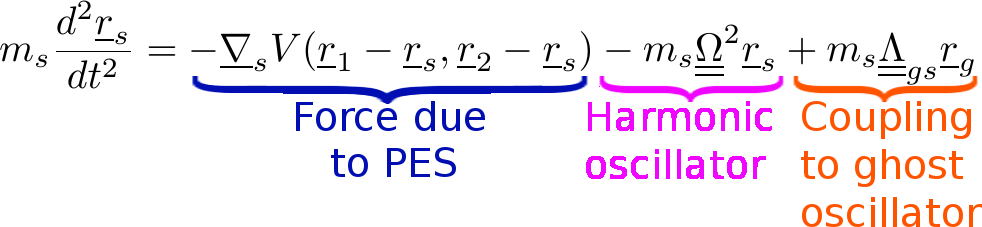
\includegraphics[width=2.6\textwidth]{figures/GLO_eq1.png}
	  \end{figure}
	  \begin{figure}
		\hspace*{-.7cm}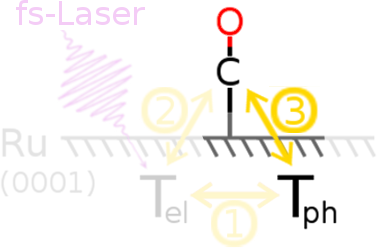
\includegraphics[width=1.3\textwidth]{figures/Part3SurfScheme.png}
	  \end{figure}
	  \vspace{-1cm}
	  \begin{figure}
		\hspace*{-.7cm}
\includegraphics[width=2.4\textwidth]{figures/GLO_eq2.png}
	  \end{figure}
	\column{.68\textwidth}
% 	  \begin{figure}
		\hspace*{-.7cm}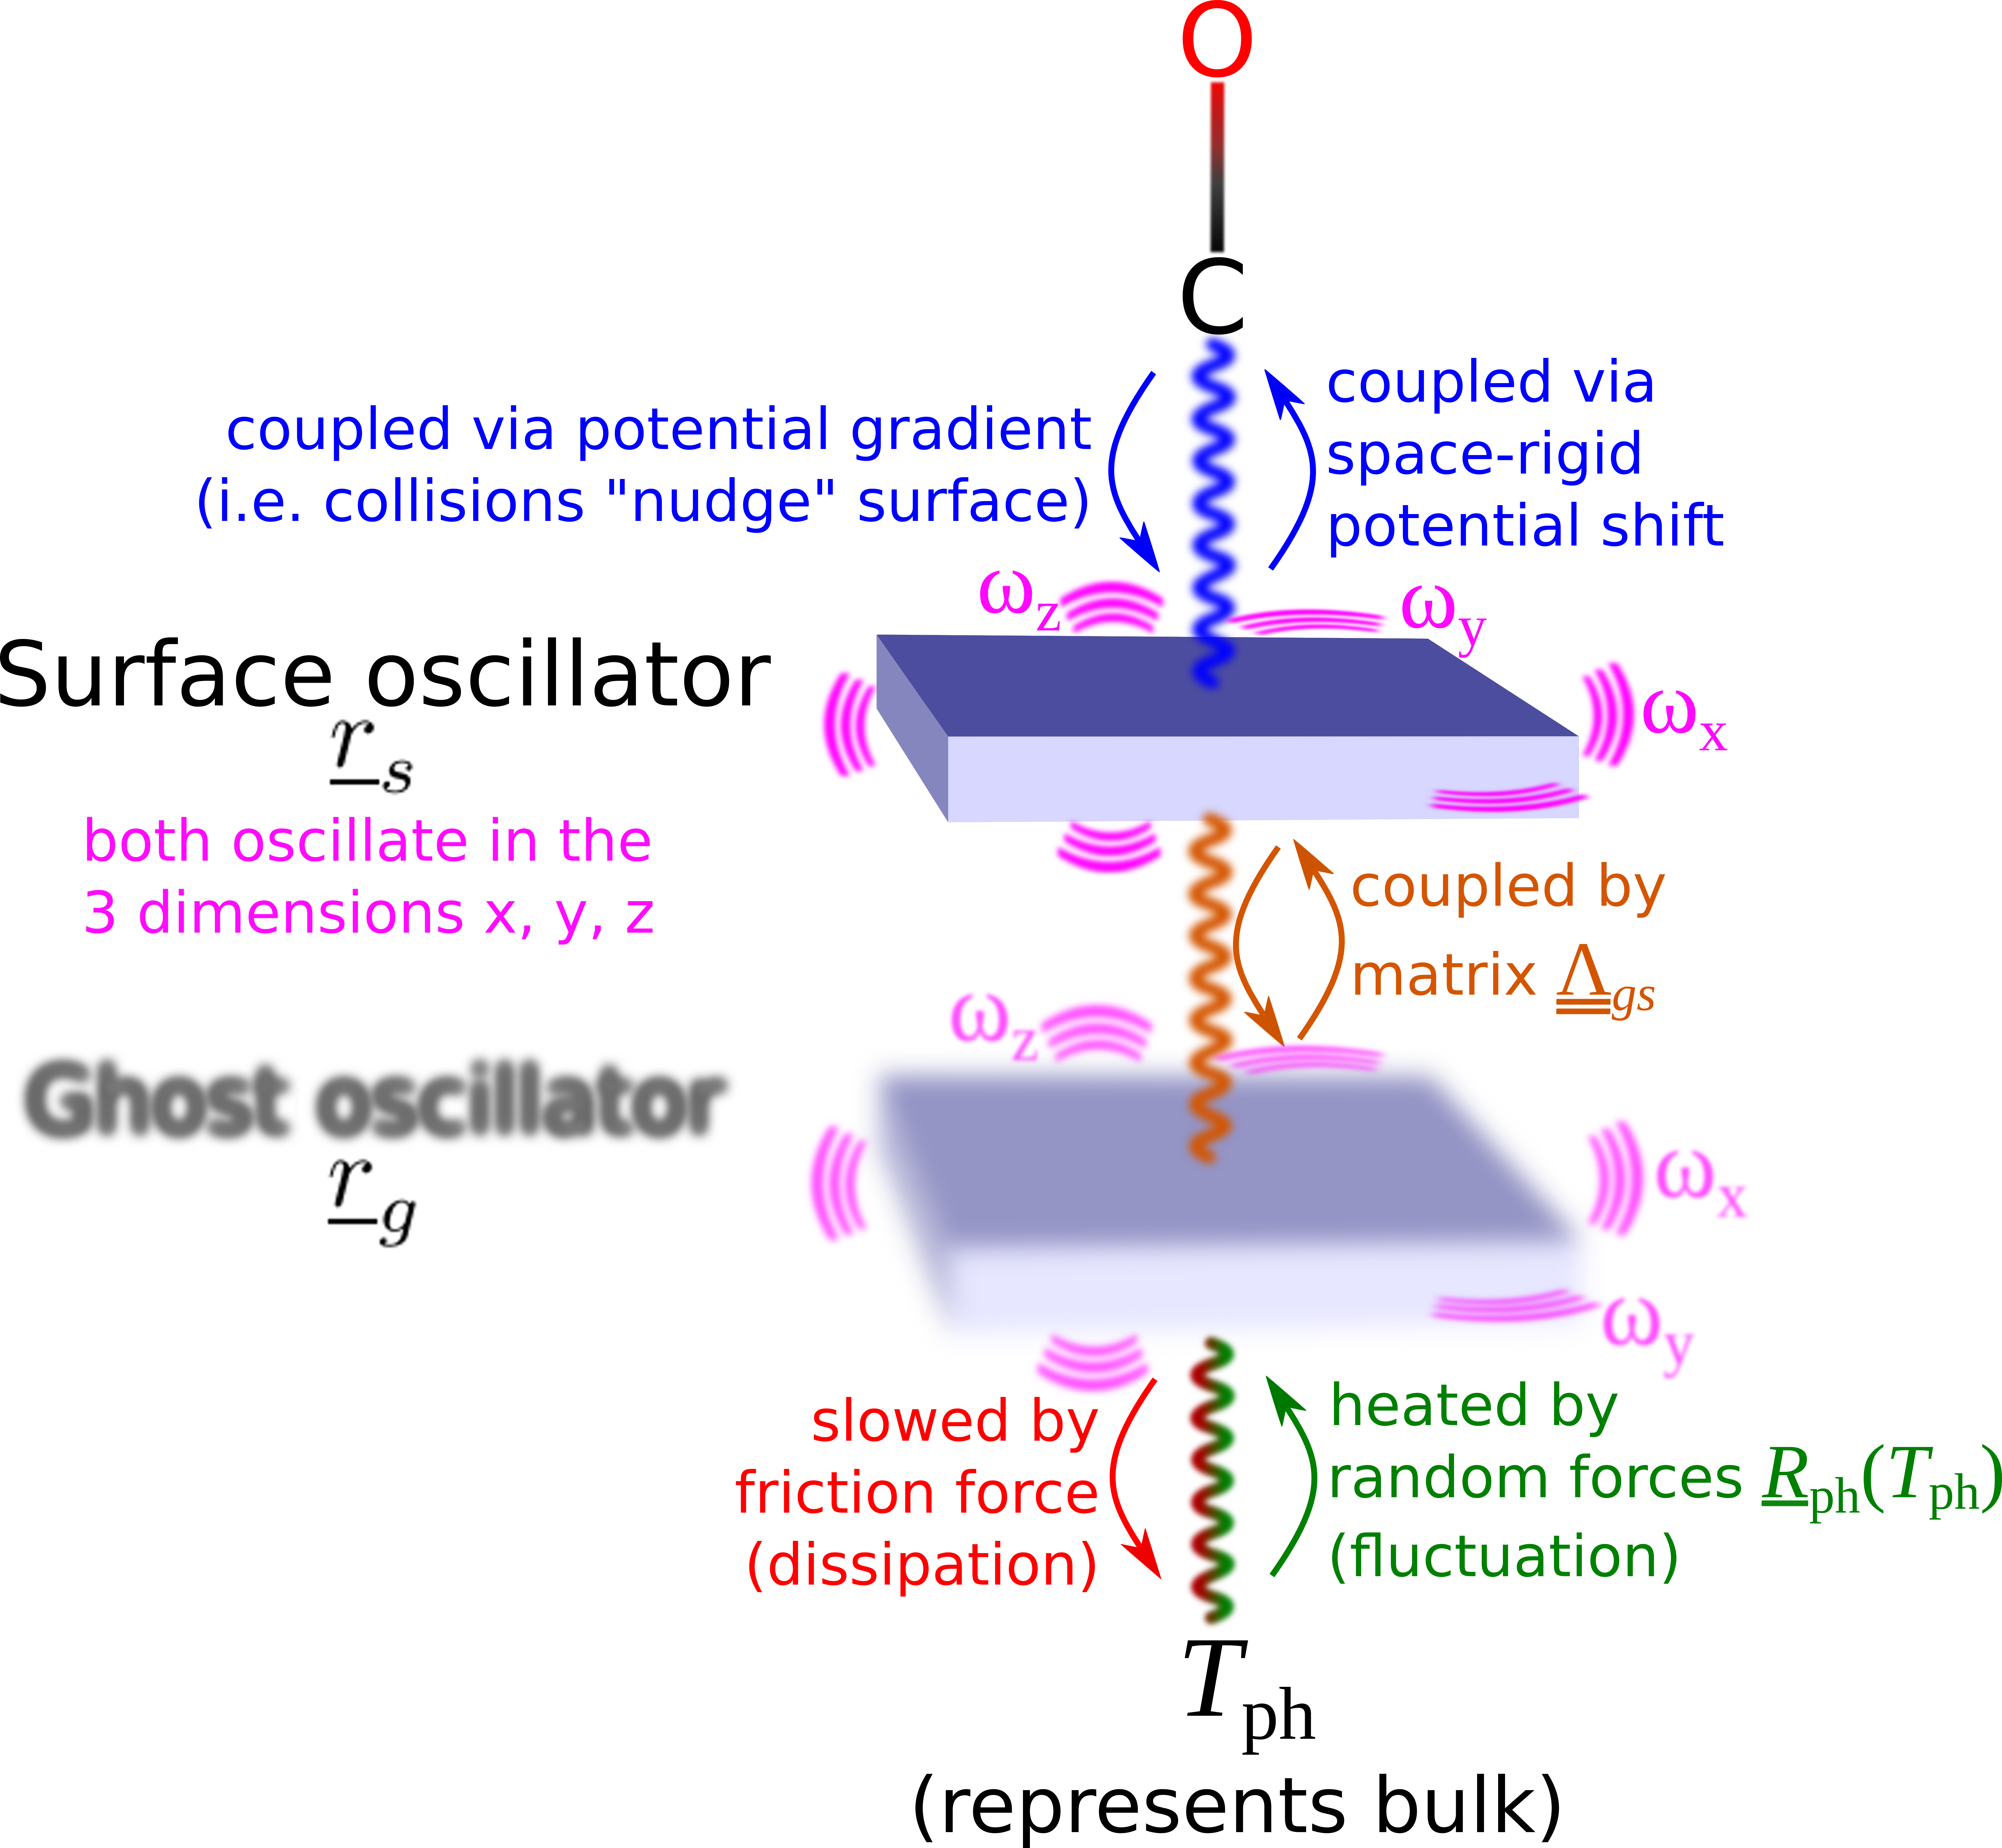
\includegraphics[width=1.2\textwidth]{figures/GLO.png}
% 	  \end{figure}
  \end{columns}
\end{frame}

\subsection[Half-time]{``Half-time'': short summary {\scriptsize(and maybe time for a few questions)}}

\begin{frame}{Summary of models and methods}
  \begin{figure}
	\hspace*{-.85cm}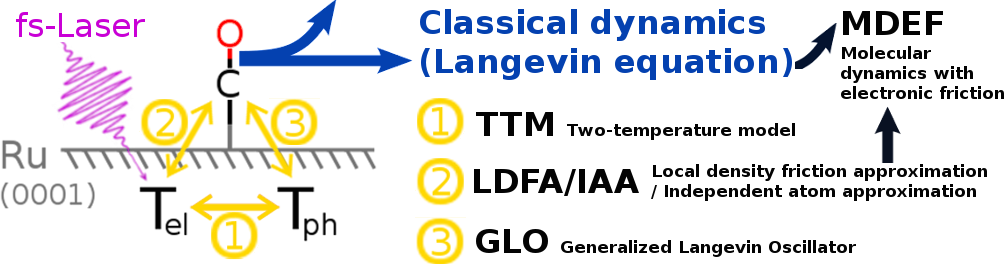
\includegraphics[width=1.15\textwidth]{figures/SummSurfScheme.png}
  \end{figure}
\end{frame}


\section{Results and discussion}

% \subsection{Overview of computational settings}
% 
% \begin{frame}{Overview of computational settings}
%   \begin{figure}
% % 	\includegraphics[width=\textwidth]{figures/}
%   \end{figure}
% \end{frame}

\subsection{Laser-driven diffusion and desorption}

\begin{frame}{Example trajectory}{(in this case without GLO-model)}
  \begin{figure}
	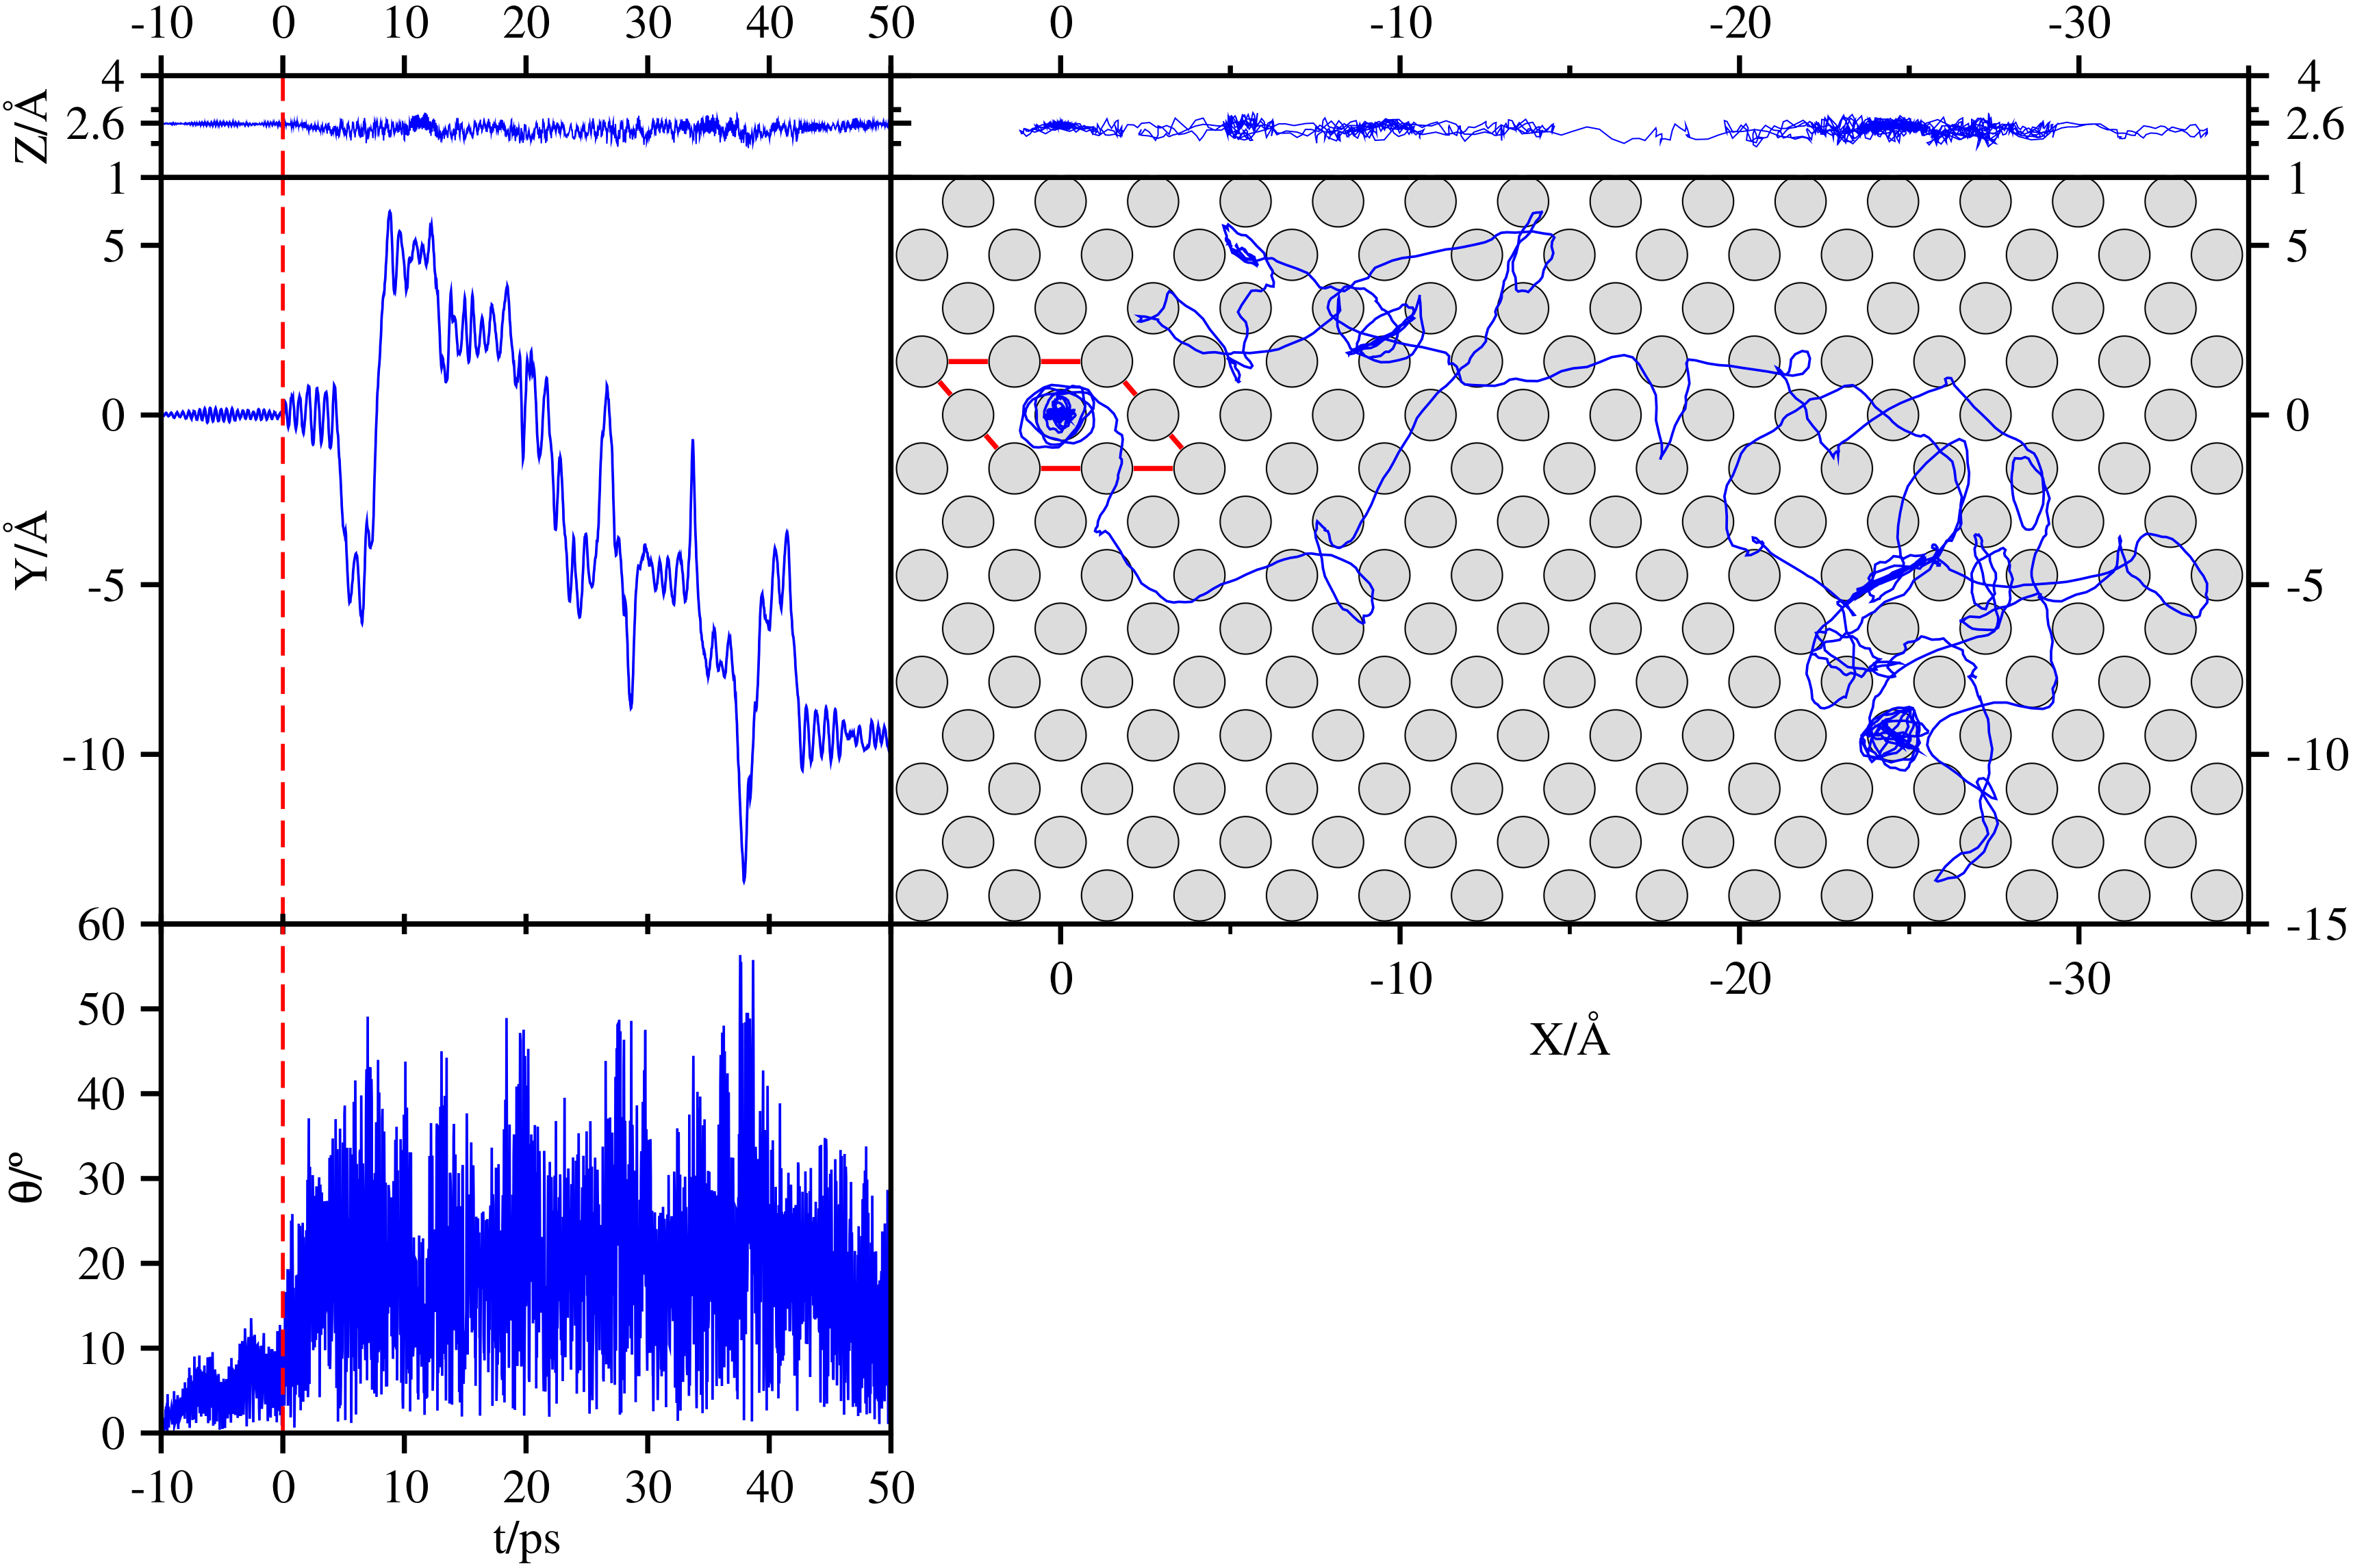
\includegraphics[width=\textwidth]{figures/Traj_XYZTh.png}
  \end{figure}
\end{frame}

\begin{frame}{Heating of DOFs $Z$ and $\theta$}
  \begin{figure}
	\vspace*{-.4cm}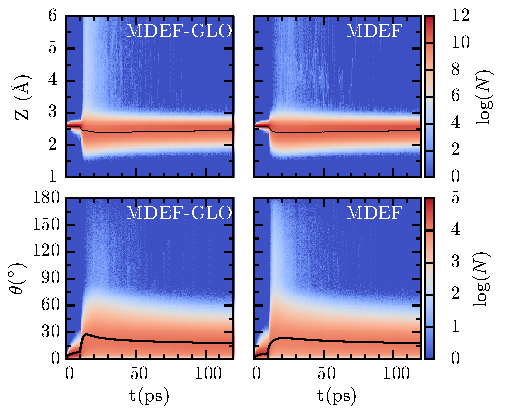
\includegraphics[width=.9\textwidth]{figures/ZundTheta.pdf}
  \end{figure}
\end{frame}

\begin{frame}{Fluence-dependence of desorption yield $P_\mathrm{des}$}
  \begin{columns}
    \column{.75\textwidth}
    \begin{figure}
      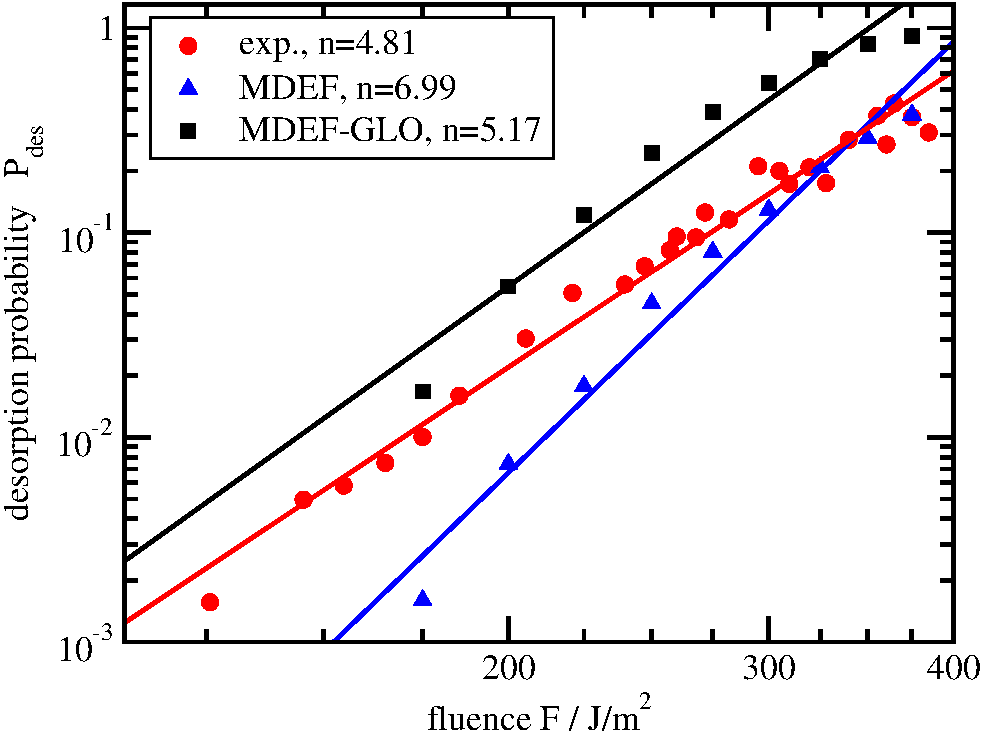
\includegraphics[width=1\textwidth]{figures/Pdes_vs_Fluence.pdf}
    \end{figure}
    \column{.3\textwidth}
      \begin{block}{Power-law}
	\begin{itemize}
	 \item $P_\mathrm{des} = A \cdot F^n$
	 \item not exactly
	\end{itemize}

      \end{block}
      
      \begin{block}{Differences in exp.}
	\begin{itemize}
	 \item coverage:
	 \item  [$\Rightarrow$] \begin{small}0.68 ML (max.)	                                      \end{small}
	\end{itemize}

      \end{block}

  \end{columns}
\end{frame}

% \begin{frame}{Two-pulse correlation of desorption}
%   \begin{figure}
% 	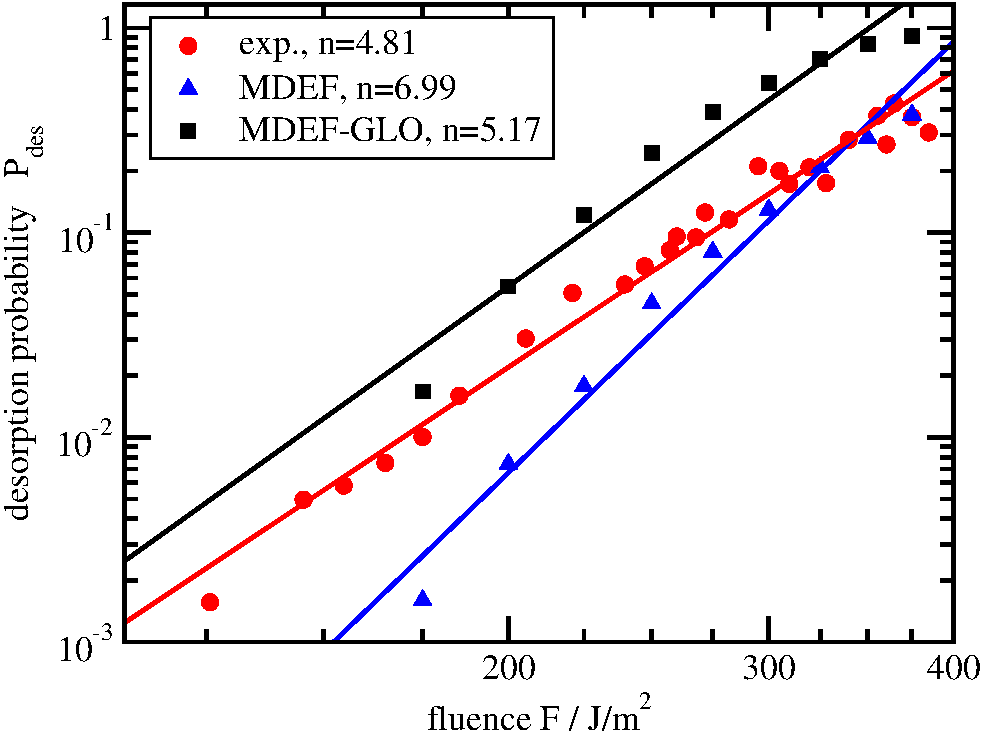
\includegraphics[width=.7\textwidth]{figures/Pdes_vs_Fluence.pdf}
%   \end{figure}
% \end{frame}

\subsection{Physisorbed precursor states?}

\begin{frame}{No population of physisorbed state in our dynamics}{As is to be expected from negligible barrier in potential of mean force (PMF)}
  \begin{columns}
  \column{0.6\textwidth}
    \begin{figure}
      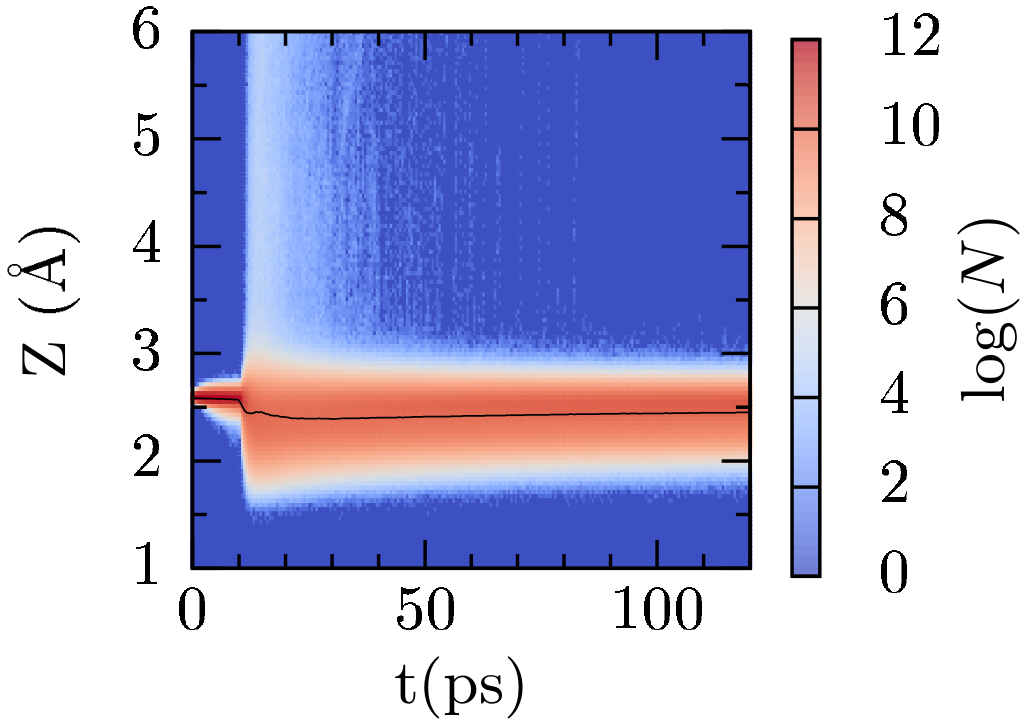
\includegraphics[width=1.\textwidth]{figures/NurZ.png}
    \end{figure}
  \column{0.4\textwidth}
    \begin{figure}
      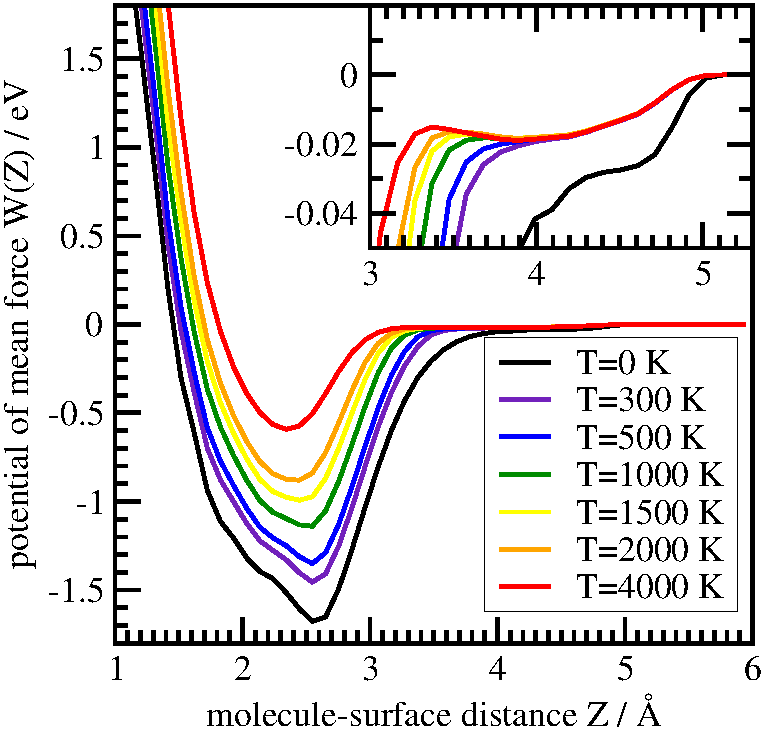
\includegraphics[width=1.\textwidth]{figures/GernotPMF.pdf}
    \end{figure}
  \end{columns}
\end{frame}

\begin{frame}{Why are the entropic barriers of the PMFs so different?}
  \begin{block}{Because separability assumption fails clearly}
    \begin{itemize}
     \item if introduced for our PMF $\Rightarrow$ barrier of similar heigth!
     \item expectable, because $X/Y$ and $\theta$ strongly coupled
    \end{itemize}
  \end{block}
  \begin{columns}
    \column{0.5\textwidth}
    \begin{figure}
      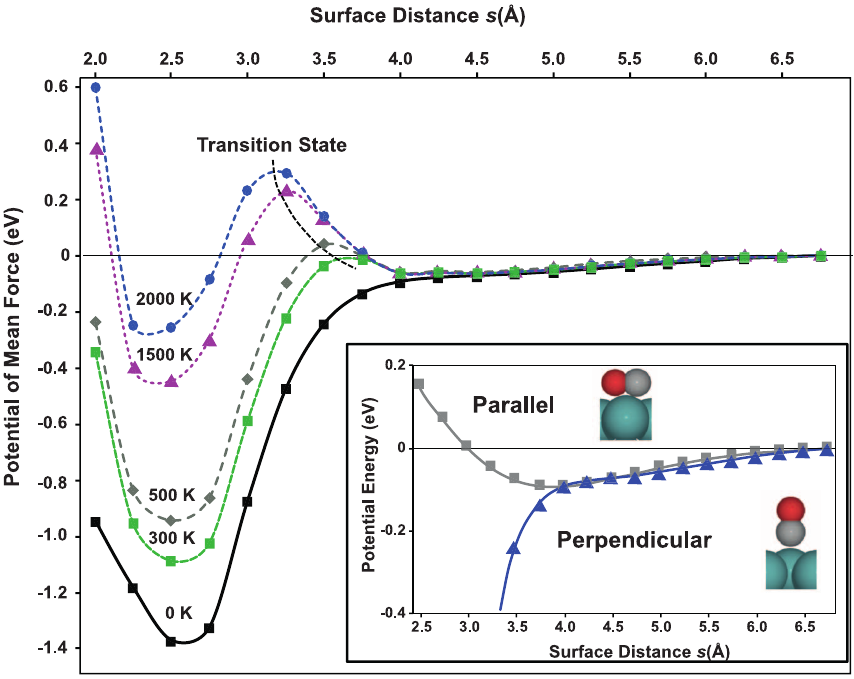
\includegraphics[width=\textwidth]{figures/sciencePMF.png}
    \end{figure}
    \column{0.5\textwidth}
    \begin{figure}
      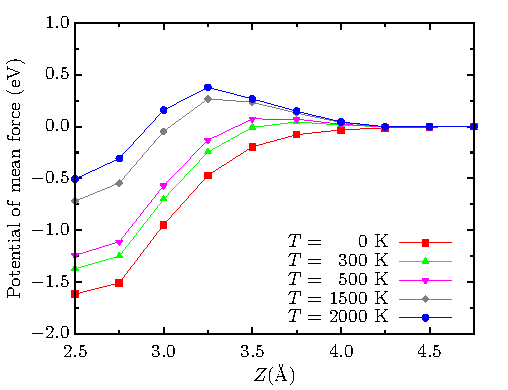
\includegraphics[width=\textwidth]{figures/PMF_Supp.pdf}
    \end{figure}   
  \end{columns}
\end{frame}



\begin{frame}{Dynamical trapping: {\normalsize alternative/additional explanation?}}

%     \begin{figure}
      \hspace*{-.6cm}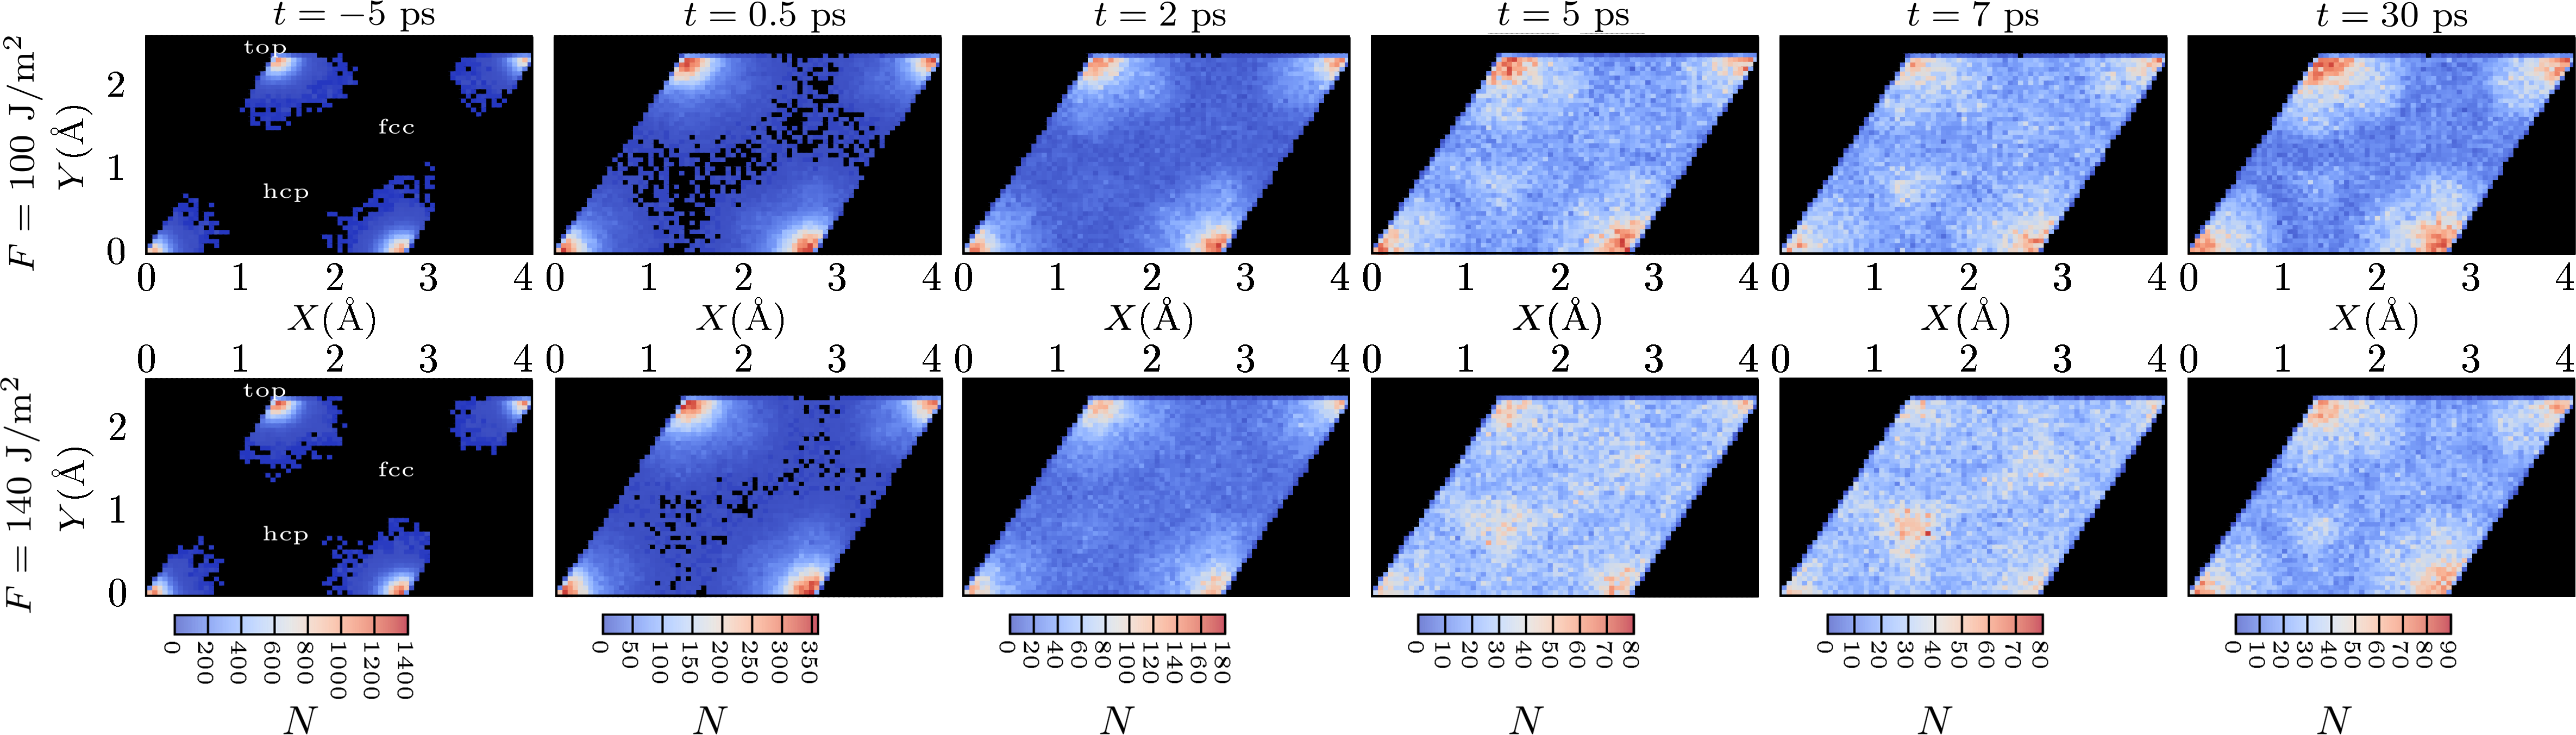
\includegraphics[width=1.1\textwidth]{figures/XYoverTime.png}
%     \end{figure}
\vspace*{-.5cm}
      \begin{columns}[t]
  \column{.65\textwidth}
  \begin{block}{Suprising patterns in XY-distribution}
    \begin{itemize}	  
      \item preferation of \textbf{hcp-site} after 5-7$\,$ps,
%       \item[$\Rightarrow$] 
      \newline despite it being a local maximum!
      \newline \textbf{$\Rightarrow$ dynamical trapping} {\footnotesize(cf. 30$\,$ps)}
      \item effect dependent on fluence
      \newline $\Rightarrow$ consistent with experiment \newline{\footnotesize(weaker ``precursor''-signal for lower fluence)}
    \end{itemize}   
  \end{block}

  \column{.4\textwidth}
    \begin{figure}
      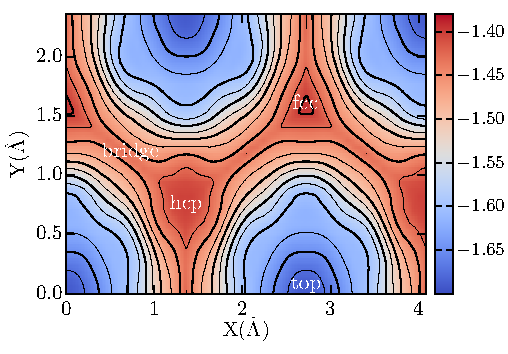
\includegraphics[width=\textwidth]{figures/PES_XYview.pdf}
    \end{figure}
  \end{columns}  
\end{frame}

\begin{frame}{Is there a physisorbed precursor state nevertheless?}
  \begin{columns}
    \column{0.7\textwidth}
    \begin{figure}
      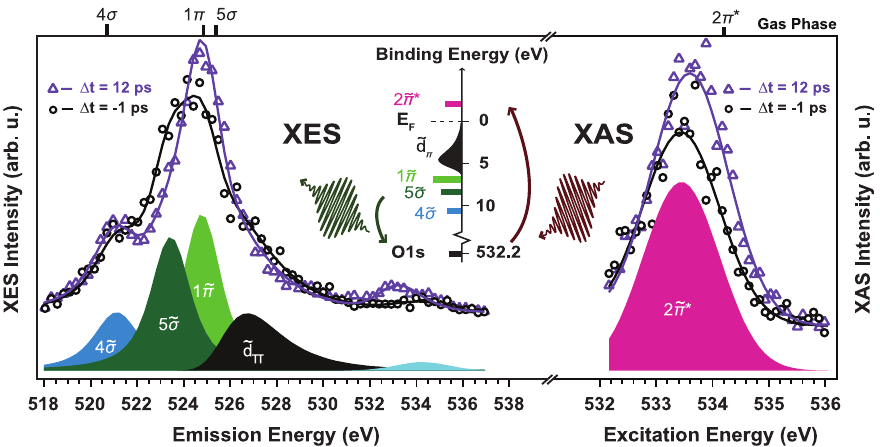
\includegraphics[width=1.\textwidth]{figures/scienceXray.png}
    \end{figure}      
    \column{0.2\textwidth}
    \begin{figure}
      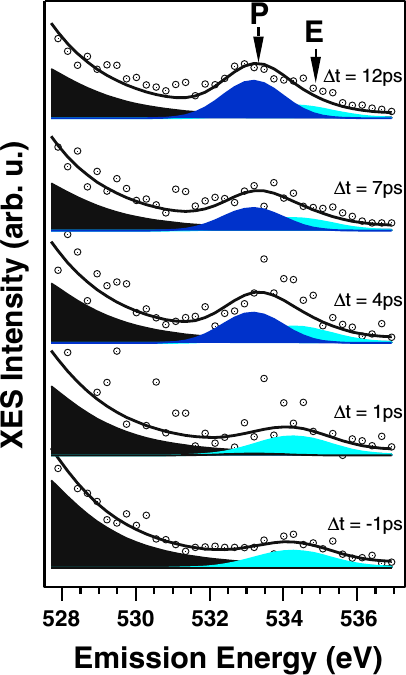
\includegraphics[width=1.\textwidth]{figures/PartiPeak.png}
    \end{figure} 
  \end{columns}
    \begin{block}{Dynamical trapping can't explain all observations}
      \begin{itemize}
        \item XAS of hcp-site: 2$\pi^*$-intensity not increased {\scriptsize(computed by Christopher)}
	\item participator peak not explained by any XY-redistributions
	\newline $\Rightarrow$ Existence of physisorbed state very likely
	  \item but nevertheless not stable for Ru(2x2):CO models 
	 \newline $\Rightarrow$ probably stabilized by CO-CO-interactions 


	
      \end{itemize}
    \end{block}
\end{frame}


\section{Summary and Outlook}

  \begin{frame}[plain]{Outline}
    \tableofcontents[currentsection]
  \end{frame}

\begin{frame}{Summary}
  \begin{block}{What was done?}
   \begin{itemize}
    \item 6D Langevin dynamics of CO @ Ru(0001)
    \begin{itemize}\scriptsize
    \item electronic friction and excitation by hot e-h-pairs (via LDFA/IAA)
    \item substrate motion (via GLO)
    \item based on ab-initio potential and first-principles, no ``free parameters''
    \end{itemize}  
   \end{itemize}

  \end{block}

  \begin{figure}
	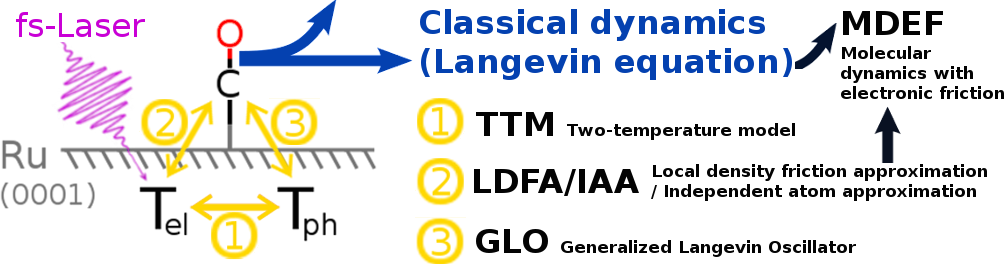
\includegraphics[width=0.85\textwidth]{figures/SummSurfScheme.png}
  \end{figure}
  \begin{block}{What could be learned?}
   \begin{itemize}
    \item detailed time- and space-resolved insight 
    \item physisorbed precursor state not stable in current model
   \end{itemize}

  \end{block}

  
\end{frame}

\begin{frame}{Outlook}{What can be done in the future?}
  \begin{block}{On the CO/Ru-system}
     \begin{itemize}
      \item better TTM, {\footnotesize with accurate $\kappa(T_\mathrm{el}, T_\mathrm{ph})$ and $g(T_\mathrm{el}, T_\mathrm{ph})$ (e-e-scattering) }  
      \item better friction model, {\footnotesize  e. g. LDFA with Atoms in Molecules (AIM)}
      \item use AIMDEF {\footnotesize to revisit short timescales of phonon-adsorbate coupling predicted by GLO}
      \item include CO-CO-interactions, \newline {\footnotesize e. g. via tailored FF for electrostatic and VdW-interactions \newline$\Rightarrow$ also enables simulation of other coverages} 
     \end{itemize}
   
  \end{block}
  \begin{block}{MDEF/GLO and AIMDEF on other systems}
    e.g. NO/Au(111), H$_2$/Au(111) etc.
  \end{block}

  
\end{frame}

\begin{frame}{Acknowledgements}
  \begin{block}{I want to thank...}
    \begin{itemize}
     \item Peter, {\footnotesize for all his support and particularly for writing the paper}
     \item Gernot, {\footnotesize for his amazing work on the PES }
     \item Ivor, {\footnotesize for everything GLO related and much more}
     \item AG Saalfrank, {\footnotesize for the pleasing atmosphere, especially ``Spa\ss{}raum 2'' } 
     \item Jan, and Martin K\"argell (HZB Wannsee),
     \newline {\footnotesize  for ideas and some much needed help}
     \item the FHI Berlin and it's IMPRS, {\footnotesize for my scholarship }
    \end{itemize}  
  \end{block}
\end{frame}



\end{document}
